\documentclass[]{beamer}
\usepackage{tikz,lstautogobble,listings}
\usetikzlibrary{arrows.meta}
\usetheme{Rochester}
\usepackage[T1]{fontenc}
\usepackage[utf8]{inputenc}
\lstset{
  language=caml,
  basicstyle=\ttfamily\tiny,
  breaklines=true,
  autogobble=true,
}


\title{TIPE 25/26 - Cycles et Boucles}
\author{GIL Dorian}
\subtitle{Méthode des tableaux : Optimisation et étude de la satisfiabilité de formule}
\date{}

\begin{document}

\begin{frame}
\titlepage
\end{frame}

\begin{frame}{Sommaire}
\begin{enumerate}
    \item Introduction Générale et Objectifs
    \item Etude Préliminaire: Forme Alternée
   
    \item Objectifs futurs
\end{enumerate}
\end{frame}

\begin{frame}{Introduction - Definition}
    \begin{definition}[Méthode des tableaux]
        Algorithme pour prouver qu'une assertion $\phi$ ayant pour hypothèse $(H_n)$ soit satisfiable
    \end{definition}
    On supposera que aucune hypothèse n'est faite, on peut facilement adapter l'étude que l'on va faire lors d'ajout d'hypothèse.
    \pause
    \begin{itemize}
        \item On place $\phi$ et ses hypothèses dans la racine.
        \item On applique des règles $(R_x)$ à chaque formule en bout d'arbre qui sont developpables
        \item Si on trouve des contradictions (des \textit{cycles}) dans toutes les branches de l'arbre (branches fermées), l'arbre est fermé donc la formule est insatisfiable.
    \end{itemize}
    \pause
    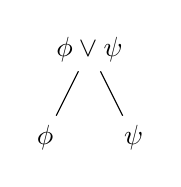
\begin{tikzpicture}[scale=0.75]
    \node {$\phi\lor\psi$}
        child {node {$\phi$}}
        child {node {$\psi$}};
    \end{tikzpicture}
    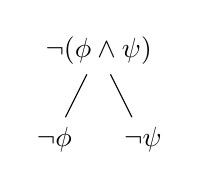
\begin{tikzpicture}[scale=0.75]
    \node {$\lnot(\phi\land\psi)$}
        child {node {$\lnot\phi$}}
        child {node {$\lnot\psi$}};
    \end{tikzpicture}
    \begin{tikzpicture}[scale=0.75]
    \node {$\lnot\lnot\phi$}
        child {node {$\phi$}};
    \end{tikzpicture}
    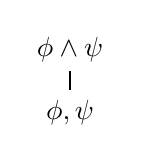
\begin{tikzpicture}[level distance=8mm]
    \node {$\phi\land\psi$}
        child {node {$\phi, \psi$}};
    \end{tikzpicture}  
    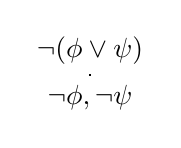
\begin{tikzpicture}[level distance=8mm,scale=0.75]
    \node {$\lnot(\phi\lor\psi)$}
        child {node {$\lnot\phi, \lnot\psi$}};
   \end{tikzpicture}
\end{frame}


\begin{frame}{Introduction - Definition}
    Les règles définis précedemment sont dites Smullyan-Style

    \begin{definition}[Branche fermée]
        Une branche est fermée si elle contient $\phi$ et $\lnot\phi$
    \end{definition}
    Une formule est insatisfisable ssi son arbre associé est dit fermé ssi toutes les branches le sont.
\end{frame}

\begin{frame}{Introduction - Remarques}
    \begin{itemize}
        \item On peut utiliser la méthode des tableaux pour montrer qu'une formule est une tautologie:
        \begin{enumerate}
            \item On place $\lnot\phi$ et ses hypothèses dans la racine.
            \item On applique des règles $(R_x)$ à chaque formule en bout d'arbre qui sont developpables
            \item Si on trouve $a$ et $\lnot a$ dans les branches de l'arbre (des \textit{cycles}), alors $\phi$ est une tautologie
        \end{enumerate}
        On pourra donc aussi adapter nos recherches pour la recherche de tautologie.
        
        \item Nous allons maintenant introduire un type de formule et étudier la méthode des tableaux sur ce cas particulier, pour en déduire des propriétés interessantes.
        Ou même des optimisations de cette méthode.
    \end{itemize}
\end{frame}

\begin{frame}{Alternée - Definition}
    \begin{definition}[Forme Alternée]
        Soit $n\in\mathbb{N}^*$, et $(a_k)_{k\in [|1,n|]}$ des litteraux, on dit que $\varphi$ est de forme alternée ssi
        $$\varphi = a_1\land(a_2\lor(a_3\land(\dots(a_n))))$$
    \end{definition}
    \pause
    On remarquera le parenthesage qui enlève toute ambiguité sur la prioritée entre les opérateurs logiques.
\end{frame}

\begin{frame}{Alternée - Propriétés}
    \begin{theorem}[Forme Negative]
        $\varphi$ une forme alternée: 
        $$\lnot\varphi = \lnot a_1\lor(\lnot a_2\land(\lnot a_3 \lor(\dots(\lnot a_n))))$$
    \end{theorem}
    \pause
    \begin{theorem}
        Chaque arbre induit par la méthode des tableaux sur une forme alternée est un arbre binaire tel qu'on nomme dans les nodes les hypothèses.
    \end{theorem}
\end{frame}

\begin{frame}{Alternée - Recherche Algorithme}
    Nous recherchons maintenant un algorithme utilisant la méthode des tableaux pour trouver la satisfiabilité des formes alternées.

    Nous allons modéliser conformement à la méthode des tableaux et au dernier theorème présenté comme un arbre binaire, plus précisement en liste chainée:
    Par exemple pour $n=5$, on aura le schéma suivant:
    
    \pause
    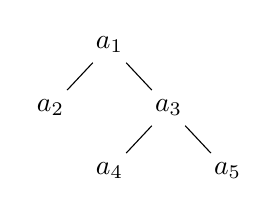
\begin{tikzpicture}[level distance=8mm]
        \node {$a_1$}
            child {node {$a_2$}}
            child {node {$a_3$}
            child {node {$a_4$}}
            child {node {$a_5$}}};
    \end{tikzpicture}
    
    \pause
    Et ce conformement au règle de la méthode des tableaux.
    La construction de cette arbre binaire se fait à priori en $\mathcal{O}(n)$
\end{frame}

\begin{frame}{Alternée - Observations}
    On va faire 3 observations, et on va en déduire un algorithme:
    \begin{itemize}
        \item Si un des litteraux dans une branche gauche (les pairs) ne provoquent aucune contradiction, c'est gagné.
        \item Dans le cas inverse, on doit rechercher plus profond dans l'arbre (parcours de la branche droite)
        \item Et ce ainsi de suite, jusqu'à en déduire un arbre fermé, ou pas
        \item Et ce en prenant aussi en compte les litteraux impairs
    \end{itemize}

    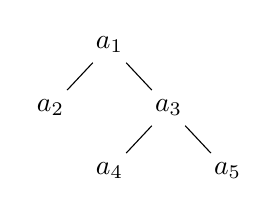
\begin{tikzpicture}[level distance=8mm]
        \node {$a_1$}
            child {node {$a_2$}}
            child {node {$a_3$}
            child {node {$a_4$}}
            child {node {$a_5$}}};
    \end{tikzpicture}
\end{frame}

\begin{frame}{Alternée - Schema Algorithme}
    On décrit un appel de l'algorithme qu'on implémente de manière recursive (dans le cas général):
    Avant cela on créé un dictionnaire. 
    On appelle litteral droit les litteraux impairs et gauche les pairs:  
    \begin{enumerate}
        \item On analyse le litteral droit, si il y a contradiction, l'arbre est fermé, sinon on ajoute eventuellement dans le dictionnaire le litteral
        \item On analyse le litteral gauche, si il produit une contradiction, appel recursif plus profond dans l'arbre, sinon la formule est satisfiable
    \end{enumerate}
    On peut montrer que cette algorithme est en $\mathcal{O}(n)$
\end{frame}

\begin{frame}{Alternée - Conséquence}
    On a donc trouvé un moyen polynomial pour montrer la satisfiabilité d'une forme alternée !!
    \pause
    \begin{itemize}
        \item En effet, ce programme est en $\mathcal{O}(n)$, c'est un parcours linéaire d'une liste chainée, utilisant des opérateurs sur les Hashtbl qu'on peut supposé constant.
        \item On prouve la terminaison: 
        \item On prouve la correction: 
    \end{itemize}
\end{frame}

\begin{frame}{Alternée - Conclusion}
    On décide de tester la vitesse d'execution de mon algorithme contre un algorithme de satisfiabilité optimisé:
    
\end{frame}


\begin{frame}{Bibliographie}
\begin{enumerate}
    \item Logique: fondements et applications (Dunod) de Pierre Le Barbenchon, Sophie Pinchinat, François Schwarzentruber
    \item Mathematical Logic: Tableaux Reasoning for Propositional Logic de Chiara Ghidini (https://dit.unitn.it/~ldkr/ml2015/slides/PLtableau.pdf)
    \item Tableau Methods  for Propositional Logic and Term Logic de Tomasz Jarmużek
\end{enumerate}
\end{frame}

\begin{frame}[fragile]{Code - Méthode des tableaux classique 1}
    \begin{center}
        \begin{tabular}{c}
            \begin{lstlisting}
                type formula =
                    | Atom of string
                    | Not of formula
                    | And of formula * formula
                    | Or of formula * formula

                let rec expand formula =
                    match formula with
                    | Not (Not f) -> [[f]]
                    | Not (And (f1, f2)) -> [[Not f1]; [Not f2]]
                    | Not (Or (f1, f2)) -> [[Not f1; Not f2]]
                    | And (f1, f2) -> [[f1; f2]]
                    | Or (f1, f2) -> [[f1]; [f2]]
                    | _ -> [];;

                let rec has_cycle branch =
                    List.exists (fun f -> List.mem (Not f) branch) branch;;
            \end{lstlisting}
        \end{tabular}
      \end{center}
\end{frame}

\begin{frame}[fragile]{Code - Méthode des tableaux classique 2}
    \begin{center}
        \begin{tabular}{c}
            \begin{lstlisting}
                let rec tableau branches =
                    match branches with
                    | [] -> false
                    | branch :: rest -> 

                    if has_cycle branch then
                        tableau rest
                    else
                        match branch with
                        | [] -> true
                        | f :: fs ->

                        let expansions = expand f in match expansions with
                        | [] -> tableau (fs :: rest)
                        | new_branches ->
                        
                        let expanded_branches = List.map (fun b -> b @ fs) new_branches in
                        tableau (expanded_branches @ rest);;

                    let is_satisfiable formula =
                    let initial_branch = [formula] in tableau [initial_branch];;
            \end{lstlisting}
        \end{tabular}
    \end{center}
\end{frame}

\begin{frame}[fragile]{Code - Alternée 1}
    \begin{center}
        \begin{tabular}{c}
            \begin{lstlisting}
                type formula =
                    | Atom of (string* bool)
                    | And of (string*bool) * formula
                    | Or of (string*bool) * formula

                type branch = 
                    | Empty
                    | Node of (formula option * formula * branch);;

                let extract (f:formula option) = match f with
                    | None ->  Atom("none", false)
                    | Some t -> t

                let rec print_formula (f:formula) = match f with
                    | Atom(s, b) -> if b then print_string s else print_string "Not ";print_string s;
                    | And ((f, b),g) -> if b then print_string f else print_string "Not ";print_string f;print_string " And ";print_formula g
                    | Or ((f,b),g) -> if b then print_string f else print_string "Not ";print_string f;print_string " Or ";print_formula g;;

                let rec print_branches (b:branch) =
                    print_string " [";
                    match b with
                        | Empty -> ()
                        | Node(a1, a2, b) -> print_formula@@extract a1;print_string ", ";print_formula a2;print_branches b;
                    print_string "]";; 
            \end{lstlisting}
        \end{tabular}
    \end{center}   
\end{frame}

\begin{frame}[fragile]{Code - Alternée 2}
    \begin{center}
        \begin{tabular}{c}
            \begin{lstlisting}
            let rec formula2branch (f:formula) : branch = match f with
                | And(a, Or(b, Atom(c))) -> Node(Some(Atom b), Atom a, Node(None, Atom(c), Empty))
                | And(a, Or(b, c)) ->  Node(Some(Atom b), Atom a, formula2branch c)
                | And(a, Atom(b)) -> Node(Some (Atom b), Atom a, Empty)
                | _ -> failwith "Pas alternee"
              
            let has_cycle (br:branch) : bool = 
                let rec aux (br:branch) (d:(string,bool) Hashtbl.t) : bool = match br with
                | Node(None, Atom (f, b), Empty) -> 
                  if Hashtbl.mem d f then 
                    Hashtbl.find d f = b
                  else
                    true
                | Node(Some(Atom(fg, bg)), Atom (fd, bd), Empty) -> 
                      if Hashtbl.mem d fd then
                        if Hashtbl.find d fd = bd then
                          not @@ Hashtbl.mem d fg && Hashtbl.find d fg <> bg
                        else 
                          false
                      else(
                        Hashtbl.add d fd bd;
                        not @@ Hashtbl.mem d fg && Hashtbl.find d fg <> bg)
                | Node(Some (Atom (fg, bg)), Atom (fd, bd), nb) ->
                  if Hashtbl.mem d fd then
                    if Hashtbl.find d fd <> bd then
            \end{lstlisting}
        \end{tabular}
    \end{center}   
\end{frame}

\begin{frame}[fragile]{Code - Alternée 3}
    \begin{center}
        \begin{tabular}{c}
            \begin{lstlisting}
                        false
                            else
                            if Hashtbl.mem d fg then
                                if Hashtbl.find d fg = bg then
                                true
                                else
                                aux nb d
                            else
                                true
                        else
                            (Hashtbl.add d fd bd;
                            if Hashtbl.mem d fg then
                            if Hashtbl.find d fg = bg then
                                true
                            else
                                aux nb d
                            else
                            true)
                        | _ -> failwith "Pas alternee"
                        in aux br (Hashtbl.create 100);;
          
            let is_satisfiable (f:formula) : bool = let b = formula2branch f in has_cycle b;;
            \end{lstlisting}
        \end{tabular}
    \end{center}   
\end{frame}
\end{document}